\chapter{Tests and metrics}

After the testbed implementation, tests about its performance and metrics were 
gathered in order to understand the real project effectiveness. We performed 
tests relatively two main sections: one testing the architecture 
overall responsivness and one checking the SFC implementation and efficiency.

Regarding the overall system responsivness, a metric we considered worth to 
test was the VNF start up time in a docker environment versus one virtualized 
through a common virtual machine system (in this case Virtual Box was choosen). 
To make this simulation as fair as possible, we used the same node (an 
Openstack VM vith 32GB of RAM, 8 vCPU and solid state storage) and used the same 
``boot sequence'' for both the VNFs: first we launched the Astaire framework, 
ensuring it's availability to process data and then we notified the test 
machine of the successful boot. The startup time was measured from the 
beginning of the startup command (\verb!docker run! for docker and 
\verb!VBoxManage -s! for Virtual Box) till the first TCP hit received by the 
test backend (to make things as smooth as possible, \verb!netcat! was used 
to listen to incoming TCP data).

It is worth saying that Docker metrics are generally more precise than the 
Virtual Box one: Docker allows to inspect the container and to gain startup and 
shutdown times with a precision of millseconds, while to gather this 
information for VirtualBox instances we had to use the command line utility 
\verb!time!, that registered timing with a precision of hundredths of a 
second. Nonetheless, this didn't influence the test too much. To avoid possible 
outliers we perfomed the test $100$ times. With this $N$, the total time spent 
by the Virtual Machines to boot up was of $2000$\todo{Update with the real 
value} seconds, while with containers the same number of start ups resulted in a 
total of $1.xx$\todo{Update with the real value}. % Insert graphs, explain the 
%problems of virtual machines
\begin{figure}[t] % TODO set subfigure and put the pie plot on the right!
 \centering
 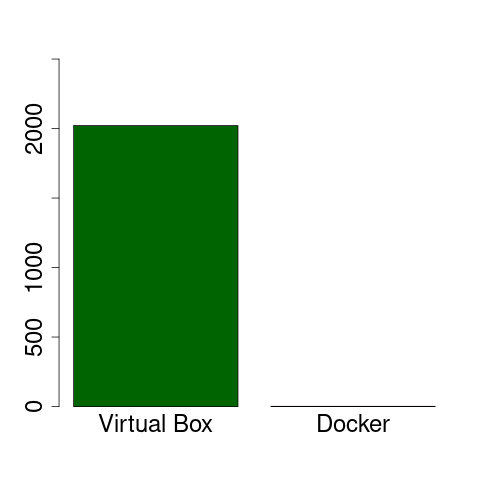
\includegraphics[scale=0.5]{docker_vs_vmBarplotGraph}
 \caption[Docker vs Virtual Box barplot results]{Docker vs Virtual Box barplot 
results. It is possible to see how the total time to start up a virtual machine 
through Virtual Box is very high compared to the time required to the overall 
Docker containers to boot. A single VirtualBox instance requires on average 20 
seconds to boot up, while a container requires, on average, only 0.02 seconds. 
The main reason behind this difference, as already explained in other parts of 
this thesis, it is caused by the guest's kernel that has to initialized itself, 
before starting any program. On Docker, instead, the kernel is the same of the 
host, so the only operations needed are to isolate the program from the rest of 
the OS and add it to the process list.}
 \label{chap:tests:sec:dockervsvb:img:barplot}
\end{figure}


% Talk about the next test
